% !TeX spellcheck = it_IT
% !TeX root = ../it.tex

\chapter{Teoria della Calcolabilità}

\section{Notazione}

\subsection{Funzioni}

\paragraph{Funzione:} Una funzione $f$ dall'insieme $A$ all'insieme $B$ è una legge che dice come associare a ogni elemento di $A$ un elemento di $B$. Si scrive
$$ f: A \rightarrow B $$
E chiamiamo $A$ dominio e $B$ codominio. Per dire come agisce su un elemento si usa $f(a) = b$, $b$ è l'immagine di $a$ secondo $f$ (di conseguenza $a$ è la controimmagine).\\
Per definizione di funzione, è possibile che elementi del codominio siano raggiungibili da più elementi del dominio, ma non il contrario. Possiamo classificare le funzioni in base a questa caratteristica:
\begin{itemize}
	\item \textbf{Iniettiva:} $f: A \rightarrow B$ è iniettiva sse $\forall a,b \in A$, $a \neq b \implies f(a) \neq f(b)$
	\item \textbf{Suriettiva:} $f: A \rightarrow B$ è suriettiva sse $\forall b \in B$, $\exists a \in A: f(a) = b$: un altro modo per definirla è tramite l'insieme immagine di $f$, definito come
	$$ \ImSet_f = \{b \in B: \exists a, f(a) = b \} = \{f(a): a \in A \} $$
	Solitamente $\text{Im}_f \subseteq B$, ma $f$ è suriettiva sse $ \ImSet_f = B$;
	\item \textbf{Biettiva:} $f: A \rightarrow B$ è biettiva sse è sia iniettiva che suriettiva, ovvero
	$$
	\begin{array}{c l}
		\forall a, b \in A, a \neq b: & f(a) \neq f(b) \\
		\forall b \in B, \exists a \in A: & f(a) = b
	\end{array}
	\implies \forall b \in B, \exists! a \in A: f(a) = b
	$$
\end{itemize}

\paragraph{Inversa:} Per le funzioni biettive si può naturalmente associare il concetto di "inversa": dato $f: A \rightarrow B$ biettiva, si definisce inversa la funzione $f^{-1}: B \rightarrow A$ tale che $f^{-1} (b) = a \Leftrightarrow f(a) = b$.\\

\paragraph{Composizione di funzioni:} Date $f: A \rightarrow B$ e $g: B \rightarrow C$, $f$ composto $g$ è la funzione $g \circ f: A \rightarrow C$ definita come $g \circ f(a) = g(f(a))$. Generalmente non commutativo, $f \circ g \neq g \circ f$, ma è associativo.\\

\paragraph{Funzione identità:} Dato l'insieme $A$, la funzione identità su $A$ è la funzione $i_A: A \rightarrow A$ tale che $i_A (a) = a$, $\forall a \in A$.\\

Un'altra possibile definizione per l'inversa diventa:
$$ f^{-1} \circ f = i_A \wedge f \circ f^{-1} = i_B $$

\paragraph{Funzioni Parziali:} Se una funzione $f: A \rightarrow B$ è definita per $a \in A$ si indica con $f(a) \downarrow$ e da questo proviene la categorizzazione: una funzione è \textbf{totale} se definita $\forall a \in A$, \textbf{parziale} altrimenti (definita solo per qualche elemento di $A$).\\

\paragraph{Insieme Dominio:} Chiamiamo \textbf{dominio} (o campo di esistenza) di $f$ l'insieme
$$ \Dom_f = \left\{a \in A | f(a) \downarrow \right\} \subseteq A $$
Quindi se $\Dom_f = A$ la funzione è totale, se $\Dom_f \subsetneq A$ allora è una funzione parziale.\\

\paragraph{Totalizzazione:} Si può \textbf{totalizzare una funzione parziale} $f$ definendo una funzione a tratti $\overline{f}: A \rightarrow B \cup \{\bot\}$ tale che
$$ 
\overline{f} (a) = \begin{cases}
	f(a) & a \in \Dom_f(a) \\
	\bot & \text{altrimenti}
\end{cases}
$$
Dove $\bot$ è il \textbf{simbolo di indefinito}, per tutti i valori per cui la funzione di partenza $f$ non è definita. Da qui in poi $B_\bot$ significa $B \cup \{\bot\}$.\\

\paragraph{Insieme delle funzioni:} L'insieme di tutte le funzioni che vanno da $A$ a $B$ si denota con
$$ B^A = \{f: A \rightarrow B \} $$
La notazione viene usata in quanto la cardinalità di $B^A$ è esattamente $|B|^{|A|}$, con $A$ e $B$ insiemi finiti.\\
Volendo includere anche tutte le funzioni parziali: 
$$ B^A_\bot = \{f: A \rightarrow B_\bot \} $$
Le due definizioni coincidono, $B^A = B^A_\bot$, ma quest'ultima permette di mettere in evidenza che tutte le funzioni presenti sono totali o totalizzate.\\ 

\subsection{Prodotto Cartesiano}

Chiamiamo \textbf{prodotto cartesiano} l'insieme 
$$ A \times B = \{(a,b) | a \in A \wedge b \in B \} $$
Rappresenta l'insieme di tutte le coppie ordinate di valori in $A$ e $B$. In generale non è commutativo, a meno che $A=B$.\\

Può essere esteso a $n$-uple di valori:
$$ A_1 \times \dots \times A_n = \{(a_1, \dots, a_n) | a_i \in A_i\} $$
Il prodotto di $n$ volte lo stesso insieme verrà, per comodità, indicato come
$$ A \times \dots \times A = A^n $$

\paragraph{Proiettore:} Operazione "opposta", il proiettore $i$-esimo è una funzione che estrae l'$i$-esimo elemento di una tupla, quindi è una funzione
$$ \pi_i: A_1 \times \dots \times A_n \rightarrow A_i \tc \pi_i (a_1, \dots, a_n) = a_i $$
La proiezione sull'asse in cui sono presenti i valori dell'insieme $a_i$.\\

\subsection{Funzione di Valutazione}
Dati $A,B$ e $B^A_\bot$ si definisce \textbf{funzione di valutazione} la funzione
$$ \omega: \bat \times A \rightarrow B \tc \omega (f,a) = f(a) $$
Prende una funzione $f$ e la valuta su un elemento $a$ del dominio. Si possono fare due tipi di analisi su questa funzione: 
\begin{itemize}
	\item Fisso $a$ e provo tutte le $f$, ottenendo un \textit{benchmark} di tutte le funzioni su $a$
	\item Fisso $f$ e provo tutte le $a$ del dominio, ottenendo il \textit{grafico} di $f$
\end{itemize}

\section{Sistemi di Calcolo}

Vogliamo modellare teoricamente un \textbf{sistema di calcolo}; quest'ultimo può essere visto come una black box che prende in input un programma $P$, dei dati $x$ e calcola il risultato $y$ di $P$ su input $x$. La macchina restituisce $y$ se è riuscita a calcolare un risultato, $\bot$ (indefinito) se è entrata in un loop.
\begin{center}
	\begin{tikzpicture}[>=stealth, auto, node distance=2cm]
		\node [block] (C) { Calcolatore };
		\node [left=of C.west, below] (P)  {$P$};
		\node [left=of C.west, above] (x)  {$x$};
		\node [right=of C] (out)  {$y/\bot$};
		
		\draw [->] (x) -- node {} (C.169);
		\draw [->] (P) -- node {} (C.194);
		\draw [->] (C) -- node {} (out);
	\end{tikzpicture}
\end{center}

Quindi, formalmente, possiamo definire un sistema di calcolo come una funzione 
$$ \C: \prog \times \dati \rightarrow \dati_\bot $$

Possiamo vedere un sistema di calcolo come una funzione di valutazione:
\begin{itemize}
	\item i dati $x$ corrispondono all'input $a$
	\item il programma $P$ corrisponde alla funzione $f$
\end{itemize}

Formalmente, un programma $P \in \prog$ è una sequenza di regole che trasformano un dato input in uno di output, ovvero l'espressione di una funzione secondo una sintassi 
$$ P: \dati \rightarrow \dati_\bot $$
e di conseguenza $P \in \dati^{\dati}_\bot$. In questo modo abbiamo mappato l'insieme $\prog$ sull'insieme delle funzioni, il che ci permette di definire il sistema di calcolo come la funzione
$$ \C: \dati^{\dati}_\bot \times \dati \rightarrow \dati $$

Analoga alla funzione di valutazione. Con $\C(P,x)$ indichiamo la funzione calcolata da $P$ su $x$ dal sistema di calcolo $\C$, che viene detta \textbf{semantica}, ovvero il suo "significato" su input $x$.\\

Il modello solitamente considerato quando si parla di calcolatori è quello di \textbf{Von Neumann}.\\

\section{Potenza Computazionale}
Indicando con 
$$ \C (P, \_): \dati \rightarrow \dati $$
la funzione che viene calcolata dal programma $P$ (semantica di $P$).\\

La \textbf{potenza computazionale} di un calcolatore è definita come l'insieme di tutte le funzioni che quel sistema di calcolo è in grado di calcolare, ovvero
$$ F(\C) = \{\C (P, \_) | P \in \prog\} \subseteq \dati_\bot^{\dati} $$

Ovvero, l'insieme di tutte le possibili semantiche di funzioni calcolabili con il sistema $\C$. Stabilire il carattere di quest'ultima inclusione equivale a stabilire \textit{cosa può fare l'informatica}:
\begin{itemize}
	\item se $F(\C) \subsetneq \dati_\bot^{\dati}$ allora esistono compiti \textbf{non automatizzabili}
	\item se $F(\C) = \dati_\bot^{\dati}$ allora l'informatica \textit{può fare tutto}
\end{itemize}

Calcolare funzioni vuol dire risolvere problemi \textit{in generale}, a ogni problema è possibile associare una funzione soluzione che permette di risolverlo automaticamente.\\

Un possibile approccio per risolvere l'inclusione è tramite la \textbf{cardinalità} (funzione che associa ogni insieme al numero di elementi che contiene) dei due insiemi. Potrebbe però presentare dei problemi: è efficace solo quando si parla di insiemi finiti. Ad esempio, l'insieme dei numeri naturali contiene l'insieme dei numeri pari $\mathbb{P} \subsetneq \mathbb{N}$, ma $|\mathbb{N}| = |\mathbb{P}| = \infty$.\\
Serve una diversa definizione di cardinalità che considera l'esistenza di infiniti \textit{più densi di altri}.\\

\section{Relazioni di Equivalenza}
Dati due insiemi $A,B$, una relazione binaria $R$ è un sottoinsieme $R \subseteq A \times B$ di coppie ordinate. Data $R \subseteq A^2$, due elementi sono in relazione sse $(a,b) \in R$. Indichiamo la relazione tra due elementi anche con la notazione infissa $aRb$. \\

Una classe importante di relazioni è quella delle \textbf{relazioni di equivalenza}: una relazione $R \subseteq A^2$ è una relazione di equivalenza sse rispetta le proprietà di
\begin{itemize}
	\item riflessività: $\forall a \in A$, $(a,a) \in R$
	\item simmetria: $\forall a,b \in A$, $(a,b) \in R \Leftrightarrow (b,a) \in R$
	\item transitività: $\forall a,b,c \in A$, $(a,b) \in R \wedge (b,c) \in R \implies (a,c) \in R$
\end{itemize}

\subsection{Partizione indotta dalla relazione di equivalenza}
A ogni relazione di equivalenza $R \subseteq A^2$ si può associare una \textbf{partizione}, ovvero un insieme di sottoinsiemi $A_i \subseteq A$ tali che
\begin{itemize}
	\item $\forall i \in \mathbb{N}^+$, $A_i \neq \emptyset$
	\item $\forall i,j \in \mathbb{N}^+$, se $i \neq j$ allora $A_i \cap A_j = \emptyset$
	\item $\bigcup_{i \in \mathbb{N}^+} A_i = A$
\end{itemize}

La relazione $R$ definita su $A^2$ \textit{induce} una partizione $\{A_1, A_2, \dots\}$ su $A$.\\

\subsection{Classi di equivalenza e Insieme quoziente}
Dato un elemento $a \in A$, chiamiamo \textbf{classe di equivalenza} di $a$ l'insieme
$$ [a]_R = \{b \in A | (a,b) \in R \} $$
Ovvero, tutti gli elementi in relazione con $a$, chiamato \textbf{rappresentante} della classe. \\

Si può dimostrare che
\begin{itemize}
	\item non esistono classi di equivalenza vuote, per riflessività
	\item dati $a,b \in A$, allora $[a]_R \cap [b]_R = \emptyset$, oppure $[a]_R = [b]_R$, i due elementi o sono in relazione o non lo sono
	\item $\bigcup_{a \in A} [a]_R = A$
\end{itemize}

L'insieme delle classi di equivalenza, per definizione, è una partizione indotta da $R$ su $A$, detta \textbf{insieme quoziente} di $A$ rispetto ad $R$, denotato con $A / R$.\\

\section{Cardinalità}

\subsection{Isomorfismi}

Due insiemi $A$ e $B$ sono \textbf{isomorfi} (\textit{equi-numerosi}) se esiste una biezione tra essi, denotato come $A \sim B$. Chiamando $\U$ l'insieme di tutti gli insiemi, la relazione $\sim$ è $\sim \subseteq \U^2$.\\

Dimostriamo che $\sim$ è una relazione di equivalenza: 
\begin{itemize}
	\item riflessività: $A \sim A$, la biezione è data dalla funzione identità $i_A$
	\item simmetria: $A \sim B \Leftrightarrow B \sim A$, la biezione è data dalla funzione inversa
	\item transitività: $A \sim B \wedge B \sim C \implies A \sim C$, la biezione è data dalla composizione delle funzioni usate per $A \sim B$ e $B \sim C$
\end{itemize}

Dato che $\sim$ è una relazione di equivalenza, permette di partizionare l'insieme $\U$, risultando in classi di equivalenza contenenti insiemi isomorfi, ovvero con la stessa cardinalità. Possiamo quindi definire la \textbf{cardinalità} come l'insieme quoziente di $\U$ rispetto alla relazione $\sim$.\\

Questo approccio permette il \textit{confronto delle cardinalità di insiemi infiniti}, basta trovare una funzione biettiva tra i due insiemi per poter affermare che sono isomorfi.\\

\subsection{Cardinalità finita}
La prima classe di cardinalità è quella delle cardinalità finite. Definiamo la seguente famiglia di insiemi:
$$ J_n = \begin{cases}
	\emptyset & \text{ se } n = 0 \\
	\{1, \dots , n\} & \text{ se } n > 0 \\
\end{cases}$$
Un insieme $A$ ha \textbf{cardinalità finita} sse $A \sim J_n$ per qualche $n \in \mathbb{N}$; in tal caso possiamo scrivere $|A| = n$. La classe di equivalenza $[J_n]_{\sim}$ identifica tutti gli insiemi di $\U$ contenenti $n$ elementi.\\

\subsection{Cardinalità infinita}
L'altra classe di cardinalità è quella delle \textbf{cardinalità infinite}, ovvero gli insiemi non in relazione con $J_n$. Si possono dividere in \textbf{numerabili} e \textbf{non numerabili}.

\subsubsection{Insiemi numerabili}
Un insieme $A$ è numerabile sse $A \sim \mathbb{N}$, ovvero $A \in [\mathbb{N}]_\sim$. Vengono anche detti \textbf{listabili}, in quanto è possibile elencare tutti gli elementi dell'insieme $A$ tramite una funzione $f$ biettiva tra $\mathbb{N}$ e $A$; grazie ad $f$ possiamo elencare gli elementi di $A$, formando l'insieme 
$$ A = \{f(0), f(1). \dots \} $$
Ed è esaustivo, in quanto elenca tutti gli elementi di $A$.\\

Questi insiemi hanno cardinalità $\aleph_0$ (\textit{aleph}).\\

\subsubsection{Insiemi non numerabili}
Gli insiemi non numerabili sono insiemi a cardinalità infinita ma non listabili, sono "più fitti" di $\mathbb{N}$; ogni lista generata non può essere esaustiva.\\

Il più noto tra gli insiemi non numerabili è l'insieme $\mathbb{R}$ dei numeri reali.\\

\begin{theor}
	L'insieme $\mathbb{R}$ non è numerabile ($\mathbb{R} \nsim \mathbb{N}$)
\end{theor}
\begin{proof}
	Suddividiamo la dimostrazione in 3 punti: 
	\begin{enumerate}
		\item dimostriamo che $\mathbb{R} \sim (0,1)$
		\item dimostriamo che $\mathbb{N} \nsim (0,1)$
		\item dimostriamo che $\mathbb{R} \nsim \mathbb{N}$
	\end{enumerate}
	
	Per dimostrare che $\mathbb{R} \sim (0,1)$ serve trovare una biezione tra $\mathbb{R}$ e $(0,1)$. Usiamo una rappresentazione grafica: 
	\begin{itemize}
		\item disegnare una semicirconferenza di raggio $1/2$, centrata in $1/2$, quindi con diametro $1$
		\item disegnare la perpendicolare al punto da mappare che interseca la circonferenza
		\item disegnare la semiretta passante per il centro $C$ e l'intersezione precedente
	\end{itemize}
	L'intersezione tra asse reale (parallela al diametro) e semiretta finale è il punto mappato. 
	
	\begin{center}
		\begin{tikzpicture}[scale=6]
			
			% Real line
			\draw (0.4,0.5) -- (1.6,0.5);
			% Draw the semicircle
			\draw[dashed] (0.75,1) arc (180:360:0.25);
			% Draw the top line segment
			\draw (0.75,1) -- (1.25,1);
			
			% Labels
			\node[above] at (0.75,1) {0};
			\node[above] at (1.25,1) {1};
			\node[above] at (1,1) {\textit{C}};
			\node[above] at (1.5,0.5) {$\mathbb{R}$};
			
			% Paths for first red ray, semicircle and first intersection
			\path [name path=rr1] (0.9,0) -- (0.9,1);
			\path [name path=semicircle] (0.75,1) arc (180:360:0.25);
			\path [name intersections={of=rr1 and semicircle, by=i1}];
			
			% First red line
			\draw[dashed,red] (0.9,1) -- (i1);
			
			% Find point beyond, draw the paths for the red ray and real, find the intersection
			\coordinate (Beyond) at ($(i1)!-1.179!(1,1)$); 
			\path [name path=rr2] (1,1) -- (Beyond);
			\path [name path=r] (0.25,0.5) -- (1.75,0.5);
			\path [name intersections={of=rr2 and r, by=i2}];
			% Draw second red ray
			\draw[dashed,red] (1,1) -- (i2);
		\end{tikzpicture}
	\end{center}
	
	Questo approccio permette di dire che $\mathbb{R}$ è isomorfo a qualsiasi segmento di lunghezza maggiore di $0$. La stessa biezione vale anche sull'intervallo chiuso $[0,1]$ (e di conseguenza qualsiasi intervallo chiuso), usando la "compattificazione" $\mathbb{R} = \mathbb{R} \cup \{\pm \infty\}$ e mappando $0$ su $-\infty$ e 1 su $+ \infty$.\\
	
	Continuiamo dimostrando che $\mathbb{N} \nsim (0,1)$: serve dimostrare che l'intervallo $(0,1)$ non è listabile, quindi che ogni lista manca di almeno un elemento. Proviamo a "costruire" un elemento che andrà a mancare. Per assurdo, sia $\mathbb{N} \sim (0,1)$, allora possiamo listare gli elementi di $(0,1)$ come 
	$$ 
	\begin{array}{c c c c c}
		0. & a_{00} & a_{01} & a_{02} & \dots \\
		0. & a_{10} & a_{11} & a_{12} & \dots \\
		0. & a_{20} & a_{21} & a_{22} & \dots \\
		0. & \multicolumn{4}{c}{\dots}
	\end{array}
	$$
	dove con $a_{ij}$ indichiamo la cifra di posto $j$ dell'$i$-esimo elemento della lista.\\
	
	Costruiamo il numero $c = 0.c_0 c_1 \dots$ tale che
	$$ c_{i} = \begin{cases}
		2 & \text{ se } a_{ii} \neq 2 \\
		3 & \text{ se } a_{ii} = 2 \\
	\end{cases}$$
	
	Viene costruito "guardando" le cifre sulla diagonale principale, apparterrà sicuramente a $(0,1)$ ma differirà per almeno una posizione (quella sulla diagonale principale) da ogni numero presente all'interno della lista. Questo è assurdo sotto l'assunzione che $(0,1)$ è numerabile, quindi abbiamo provato che $\mathbb{N} \nsim (0,1)$.\\
	
	Il terzo punto $\mathbb{R} \nsim \mathbb{N}$ si dimostra per transitività.\\
	
	Più in generale, non si riesce a listare nessun segmento di lunghezza maggiore di 0.\\
\end{proof}

Questa dimostrazione (punto 2 in particolare) è detta \textbf{dimostrazione per diagonalizzazione}.\\

L'insieme $\mathbb{R}$ viene detto \textbf{insieme continuo} e tutti gli insiemi isomorfi a $\mathbb{R}$ si dicono continui a loro volta.\\

Gli insiemi continui hanno cardinalità $\aleph_1$.\\

%Decidi se sub o subsub
\subsubsection{Insieme delle Parti}
L'\textbf{insieme delle parti} di $\mathbb{N}$ (anche detto \textit{power set}), è definito come
$$ P(\mathbb{N}) = 2^{\mathbb{N}} = \{S | S \text{ è sottoinsieme di } \mathbb{N}\} $$

\begin{theor}
	$P(\mathbb{N}) \nsim \mathbb{N}$.\\
\end{theor}
\begin{proof}
	Possiamo dimostrare questo teorema tramite diagonalizzazione. Il vettore caratteristico di un sottoinsieme è un vettore che nella posizione $p_i$ ha 1 se $i \in A$, 0 altrimenti (tipo vettore di incidenza).\\
	
	Rappresentiamo $A \subseteq \mathbb{N}$ sfruttando il suo vettore caratteristico
	$$ \begin{array}{c c c c c c c c c}
		\mathbb{N}: & 0 & 1 & 2 & 3 & 4 & 5 & 6 & \dots \\
		A: & 0 & 1 & 1 & 0 & 1 & 1 & 0 & \dots \\
	\end{array}$$
	
	Supponiamo, per assurdo, che $P (\mathbb{N})$ sia numerabile. Vista questa proprietà, possiamo listare tutti i vettori caratteristiche che appartengono a $P(\mathbb{N})$ come
	$$ 
	\begin{array}{c c c c c c}
		b_0 & = & b_{00} & b_{01} & b_{02} & \dots \\
		b_1 & = & b_{10} & b_{11} & b_{12} & \dots \\
		b_2 & = & b_{20} & b_{21} & b_{22} & \dots \\
	\end{array}
	$$
	Vogliamo quindi costruire un vettore che appartiene a $P(\mathbb{N})$ ma non presente nella lista precedente. Definiamo
	$$ c = \overline{b_{00}} \, \overline{b_{11}} \, \overline{b_{22}} \dots $$
	ovvero il vettore che contiene in posizione $c_i$ il complemento di $b_{ii}$.\\
	
	Questo vettore appartiene a $P(\mathbb{N})$, in quanto sicuramente sottoinsieme di $\mathbb{N}$, ma non è presente nella lista precedente perché diverso da ogni elemento almeno di una cifra (quella sulla diagonale principale). \\
	
	Questo è assurdo per l'assunzione che $P(\mathbb{N})$ è numerabile, quindi $P(\mathbb{N}) \nsim \mathbb{N}$.\\
\end{proof}

\subsubsection{Insieme delle funzioni}
L'\textbf{insieme delle funzioni} da $\mathbb{N}$ a $\mathbb{N}$ è definito come
$$ \mathbb{N}^{\mathbb{N}}_\bot = \{f: \mathbb{N} \rightarrow \mathbb{N} \} $$

\begin{theor}
	$\mathbb{N}_\bot^{\mathbb{N}} \nsim \mathbb{N}$.\\
\end{theor}
\begin{proof}
	Diagonalizzazione strikes again. Assumiamo, per assurdo, che $\mathbb{N}_\bot^{\mathbb{N}}$ sia numerabile. Possiamo quindi listare $\mathbb{N}_\bot^{\mathbb{N}}$ come $\{f_0, f_1, f_2, \dots\}$
	$$
	\renewcommand{\arraystretch}{2}
	\begin{array}{|m{1cm}|m{1cm}|m{1cm}|m{1cm}|m{1cm}|m{1cm}|m{1cm}|}
		\hline
		& $0$ & $1$ & $2$ & $3$ & $\dots$ & $\mathbb{N}$ \\
		\hline
		$f_0$ & $f_0 (0)$ & $f_0 (1)$ & $f_0 (2)$ & $f_0 (3)$ & $\dots$ & $\dots$ \\
		\hline
		$f_1$ & $f_1 (0)$ & $f_1 (1)$ & $f_1 (2)$ & $f_1 (3)$ & $\dots$ & $\dots$ \\
		\hline
		$f_2$ & $f_2 (0)$ & $f_2 (1)$ & $f_2 (2)$ & $f_2 (3)$ & $\dots$ & $\dots$ \\
		\hline
		$\dots$ & $\dots$ & $\dots$ & $\dots$ & $\dots$ & $\dots$ & $\dots$ \\
		\hline
	\end{array}
	$$
	
	Costruiamo una funzione $\varphi: \mathbb{N} \rightarrow \mathbb{N}_\bot$ per dimostrare l'assurdo. Un'idea potrebbe essere $\varphi(n) = f_n(n) + 1$, "spostando" la diagonale, ma non tiene in considerazione il caso $f_n (n) = \bot$ in quanto non sapremmo dare un valore a $\varphi (n) = \bot +1$. Definiamo quindi
	$$ 
	\varphi(n) = \begin{cases}
		1 & \text{ se } f_n (n) = \bot \\
		f_n (n) + 1 & \text{ se } f_n (n) \downarrow 
	\end{cases}
	$$
	
	Questa funzione appartiene a $\mathbb{N}_\bot^{\mathbb{N}}$, ma non è presente nella lista precedente, infatti $\forall k \in \mathbb{N}$ si ottiene 
	$$ 
	\varphi(k) = \begin{cases}
		1 \neq f_k (k) = \bot & \text{ se } f_k (k) = \bot \\
		f_k(k) + 1 \neq f_k (k) & \text{ se } f_k (k) \downarrow
	\end{cases}
	$$
	
	%TODO Check?
	Questo è assurdo sotto l'assunzione che $\mathbb{N}_\bot^{\mathbb{N}}$ è numerabile, quindi $\mathbb{N}_\bot^{\mathbb{N}} \nsim \mathbb{N}$.\\
\end{proof}

\section{Potenza Computazionale di un sistema di calcolo}
\subsection{Validità dell'inclusione $F(\C) \subseteq \dati_\bot^{\dati}$}

Dopo aver dato una più robusta definizione di cardinalità, possiamo studiare la natura dell'inclusione
$$ F(\C) \subseteq \dati_\bot^{\dati} $$

Due intuizioni, da dimostrare, sono: 
\begin{itemize}
	\item $\prog \sim \mathbb{N}$: ogni programma può essere identificato con un numero, come la sua codifica in binario
	\item $\dati \sim \mathbb{N}$: anche ogni dato può essere identificato tramite la sua codifica in binario
\end{itemize}

Da questo possiamo dire che
$$ F(\C) \sim \prog \sim \mathbb{N} \nsim \mathbb{N}_\bot^{\mathbb{N}} \sim \dati_\bot^{\dati} $$

Questo dimostra che \textbf{esistono funzioni non calcolabili}, ci sono troppe funzioni e troppi pochi programmi.\\

Dobbiamo dimostrare le due assunzioni $\prog \sim \mathbb{N}$ e $\dati \sim \mathbb{N}$. Si può fare tramite tecniche di aritmetizzazione (o godelizzazione) di strutture, tecniche che rappresentano delle strutture tramite un numero.

\subsection{$\dati \sim \mathbb{N}$}
Serve trovare una legge che
\begin{enumerate}
	\item Associ biunivocamente dati a numeri e viceversa
	\item Consenta di operare direttamente sui numeri per operare sui corrispondenti dati, ovvero abbia delle primitive che permettano di lavorare sul numero che "riflettano" il risultato sul dato, senza passare dal dato stesso
	\item Consenta di dire, senza perdita di generalità, che i programmi lavorano su numeri
\end{enumerate}

\subsubsection{Funzione Coppia di Cantor}
La \textbf{funzione coppia di Cantor} è la funzione
$$ \langle , \rangle: \mathbb{N} \times \mathbb{N} \rightarrow \mathbb{N}^+ $$
E sfrutta le due "sotto-funzioni" 
$$
\begin{array}{r c}
	\sin: & \mathbb{N}^+ \rightarrow \mathbb{N} \\
	\des: & \mathbb{N}^+ \rightarrow \mathbb{N}
\end{array}
$$
Tali che 
$$ \langle x,y \rangle = n \implies \begin{array}{r c}
	\sin (n) & = x \\
	\des (n) & = y
\end{array}$$
Si può rappresentare graficamente come

\begin{center}
	\begin{minipage}[h]{0.45\textwidth}
		{\renewcommand{\arraystretch}{1.3}
			\begin{tabular}{c | c c c c c}
				$x\setminus y$ & 0 & 1 & 2 & 3 & $\dots$ \\ 
				\hline
				0 & 1 & 3 & 6 & 10 & $\dots$ \\
				1 & 2 & 5 & 9 & $\dots$ & \\
				2 & 4 & 8 & $\dots$ && \\
				3 & 7 & $\dots$ &&& \\
		\end{tabular}}
	\end{minipage}
	\hfill 
	\begin{minipage}[h]{0.45\textwidth}
		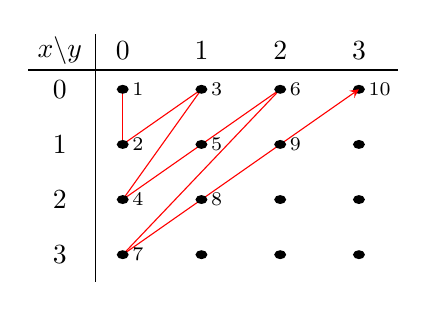
\begin{tikzpicture}[yscale=.7]
			\usetikzlibrary{arrows.meta}
			
			\tikzset{
				myarrow/.style=-stealth
			}
			
			\foreach \x in {0,1,2,3} {
				\node at (.2,-\x-1) {\x};
			}
			\foreach \y in {0,1,2,3} {
				\node at (\y+1,-.3) {\y};
			}
			\draw[red] (1,-1) -- (1,-2);
			\draw[red] (1,-2) -- (2,-1);
			\draw[red] (2,-1) -- (1,-3);
			\draw[red] (1,-3) -- (3,-1);
			\draw[red] (3,-1) -- (1,-4);
			\draw[red] (1,-4) -- (3+.2,-2+.2);
			
			\node at (.2,-.3) {$x\backslash y$};
			\foreach \x in {0,1,2,3} {
				\foreach \y in {0,1,2,3} {
					\ifthenelse{\x<\y \OR \x=\y}{
						\draw[thick,fill] (4-\y,-\x-1) circle (.06);
					}{}
				}
			}
			\draw[myarrow,red] (3+.2,-2+.2) -- (4,-1);
			\node[right] at (1,-1) {\scriptsize 1};
			\node[right] at (1,-2) {\scriptsize 2};
			\node[right] at (2,-1) {\scriptsize 3};
			\node[right] at (1,-3) {\scriptsize 4};
			\node[right] at (2,-2) {\scriptsize 5};
			\node[right] at (3,-1) {\scriptsize 6};
			\node[right] at (1,-4) {\scriptsize 7};
			\node[right] at (2,-3) {\scriptsize 8};
			\node[right] at (3,-2) {\scriptsize 9};
			\node[right] at (4,-1) {\scriptsize 10};
			
			\draw (-.2,-.65) -- (4.5,-.65);
			\draw (.65,0) -- (.65,-4.5);
			
		\end{tikzpicture}
	\end{minipage}
\end{center}

Il valore $\langle x,y \rangle$ rappresenta l'incrocio tra la $x$-esima riga e la $y$-esima colonna. Per costruirla:
\begin{enumerate}
	\item $x = 0$
	\item si parte dalla cella $(x,0)$ e si enumerano le celle della diagonale identificata da $(x,0)$ e $(0,x)$
	\item si incrementa $x$ di $1$ e si ripete dal punto precedente
\end{enumerate}

La funzione deve essere: 
\begin{itemize}
	\item iniettiva: non ci possono essere celle con lo stesso numero
	\item suriettiva: ogni numero in $\mathbb{N}^+$ deve comparire
\end{itemize}
Entrambe le proprietà sono soddisfatte, in quanto la numerazione avviene in maniera incrementale, quindi ogni numero prima o poi compare in una cella e di conseguenza ho una coppia che lo genera.\\

\paragraph{Forma analitica:} Per la definizione di $\langle x,y \rangle$ si può notare che
$$ \langle x,y \rangle = \langle x + y,0 \rangle + y $$

\begin{center}
	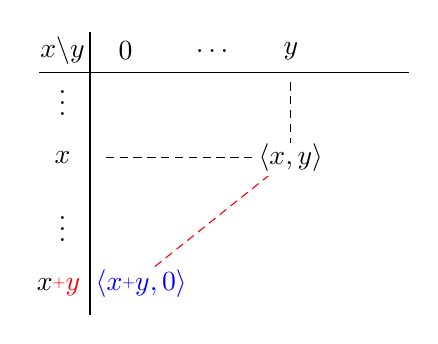
\begin{tikzpicture}[yscale=.8]
		\usetikzlibrary{arrows.meta}
		
		\newcommand{\smallerplus}{\raisebox{.3\height}{\scalebox{.6}{+}}}
		
		\draw[red,densely dashed] (1,-4) -- (3,-2);
		\draw[densely dashed] (.65,-2) -- (3,-2);
		\draw[densely dashed] (3,-1+.2) -- (3,-2);
		
		\node at (.1,-.3) {$x\backslash y$};
		
		\node at (2+1,-.3) {$y$};
		\node at (.9,-.3) {0};
		\node at (1+1,-.3) {$\dots$};
		\node at (.1,-1) {$\vdots$};
		\node at (.1,-1-1) {$x$};
		\node at (.1,-2-1) {$\vdots$};
		\node at (.05,-3-1-.05) {$x{\color{red}\smallerplus y}$};
		\def \offset {.28}
		\draw[white,fill] (3-\offset-.15,-2-\offset) rectangle (3+\offset+.05,-2+\offset-.05);
		\node at (3,-2) {$\langle x,y \rangle$};
		\draw[white,fill] (1-\offset-.15,-4-\offset) rectangle (1+\offset+.05,-4+\offset-.05);
		\node[blue] at (1.1,-4) {$\langle x \smallerplus y, 0 \rangle$};
		
		\draw (-.2,-.65) -- (4.5,-.65);
		\draw (.45,0) -- (.45,-4.5);
	\end{tikzpicture}	
\end{center}

Intuitivamente, a partire da $\langle x + y, 0\rangle$ mi basta "salire" seguendo la diagonale fino a $\langle x,y$, ovvero $y$ posti, e per definizione della funzione, $y$ valori più in alto.\\

Il calcolo della funzione coppia si può quindi ridurre al calcolo di $\langle x + y, 0$. Chiamando $x + y = z$, si può notare come ogni cella 
$$ \langle z,0 \rangle = z + \langle z - 1, 0 \rangle $$
E di conseguenza
\begin{align*}
	\langle z,0 \rangle & = z + \langle z - 1, 0 \rangle \\
	& = z + (z-1) + \langle z-2, 0 \rangle \\
	& = z + (z-1) + \dots + 1 + \langle 0,0 \rangle = \\
	& = \sum_{i=1}^{z} i + 1 = \frac{z(z+1)}{2} + 1
\end{align*}

Mettendo insieme le due proprietà viste possiamo ottenere la formula analitica per la funzione coppia: 
$$ \langle x,y \rangle = \langle x + y, 0 \rangle + y = \frac{(x + 1) (x + y + 1)}{2} + y + 1 $$

\paragraph{Forma analitica di $\sin$ e $\des$:} Vogliamo fare la stessa cosa per $\sin$ e $\des$, in modo da poter computare l'inversa della funzione coppia, dato $n$. Grazie alle osservazioni precedenti sappiamo che
$$ \begin{array}{r c l}
	\gamma = x + y & \implies & x = \gamma + y \\
	n = y + \langle \gamma , 0 \rangle & \implies & y = n - \langle \gamma , 0 \rangle \\
\end{array} $$

Trovando il valore di $\gamma$ possiamo trovare $x$ e $y$. \\

Notiamo come $\gamma$ sia il più grande valore che, quando calcolato sulla prima colonna ($\langle \gamma, 0 \rangle$) non supera $n$, ovvero
$$ \gamma = \max \{z \in \mathbb{N} | \langle z, 0 \rangle \leq n \} $$
Intuitivamente, si tratta dell'inizio della diagonale che contiene $n$, è "l'inverso" dell'osservazione fatta in precedenza per la quale $ \langle x,y \rangle = \langle x + y,0 \rangle + y $.\\

Risolviamo quindi la disequazione
\begin{align*}
	\langle z, 0 \rangle \leq n & \implies \frac{z(z+1)}{2} + 1 \leq n \\
	& \implies z^2 + z - 2n + 2 \leq 0 \\
	& \implies z_{1,2} = \frac{-1 \pm \sqrt{1 + 8n - 8}}{2} \\
	& \implies \frac{-1 - \sqrt{8n - 7}}{2} \leq z \leq \frac{-1 + \sqrt{8n - 7}}{2} 
\end{align*}

Come valore di $\gamma$ scegliamo
$$ \gamma = \left\lfloor \frac{-1 + \sqrt{8n - 7}}{2} \right\rfloor $$

E con $\gamma$ noto possiamo definire le funzioni $\sin$ e $\des$ come
$$ 
\begin{array}{r c l}
	\des(n) & = & y = n - \langle \gamma, 0 \rangle = n - \frac{\gamma (\gamma + 1)}{2} - 1 \\
	\sin (n) & = & x = \gamma - y
\end{array}
$$

\begin{theor}
	$\mathbb{N} \times \mathbb{N} \sim \mathbb{N}^+$
\end{theor}
\begin{proof}
	La funzione di Cantor è una funzione biettiva tra l'insieme $\mathbb{N} \times \mathbb{N}$ e l'insieme $\mathbb{N}^+$, quindi i due insiemi sono isomorfi.\\
\end{proof}

Possiamo estendere il risultato all'interno dell'insieme $\mathbb{N}$, ovvero:

\begin{theor}
	$\mathbb{N} \times \mathbb{N} \sim \mathbb{N}$
\end{theor}
\begin{proof}
	Definiamo la funzione 
	$$ [,]: \mathbb{N} \times \mathbb{N} \rightarrow \mathbb{N} $$
	tale che
	$$ [x,y] = \langle x,y \rangle - 1$$
	Questa funzione è anch'essa biettiva, quindi i due insiemi sono isomorfi.\\
\end{proof}

Grazie a questo è possibile dimostrare anche che $\mathbb{Q} \sim \mathbb{N}$, infatti i numeri razionali si possono rappresentare come coppie (num, den) e, in generale, tutte le tuple sono isomorfe e $\mathbb{N}$, basta iterare in qualche modo la funzione coppia di Cantor.\\

\subsubsection{Applicazione alle strutture dati}
I risultati ottenuti fin'ora rendono intuibile come ogni dato possa essere trasformato in un numero, soggetto a trasformazioni matematiche. La dimostrazione \textit{formale} non verrà fatta, anche se verranno fatti esempi di alcune strutture dati che possono essere trasformate in un numero tramite la funzione coppia di Cantor. Ogni struttura dati può essere manipolata e trasformata in una coppia $(x,y)$.\\

Le \textbf{liste} sono le strutture dati più utilizzate nei programmi. In generale non ne è nota la grandezza, di conseguenza è necessario trovare un modo, soprattutto durante l'applicazione di $\sin$ e $\des$, per capire quando abbiamo esaurito gli elementi della lista.\\

Estendiamo la funzione coppia a una lista di interi $x_1, \dots, x_n$:
$$ \langle x_1, \dots, x_n \rangle \rightarrow \langle x_1, \langle x_2 \langle \dots \langle x_n, 0 \rangle \dots \rangle \rangle \rangle $$

Lo $0$ rappresenta il fine lista e non è necessario nel caso in cui il numero di elementi è noto.\\

La decodifica è il processo inverso, partendo dal numero finale si applicano le funzioni $\sin$ e $\des$ ottenendo a ogni iterazione: 
\begin{itemize}
	\item da $\des$ la somma parziale, su cui riapplicare la funzione per ottenere il valore successivo
	\item da $\sin$ il valore presente all'interno della lista
\end{itemize} 
Termina quando il risultato di $\des$ è zero, ovvero l'elemento di fine lista che abbiamo inserito ($x_n$ nel caso di array).
\begin{center}
	\begin{tikzpicture}[
		level distance=13mm,
		sibling distance=30mm,
		]
		\node {\Large$n_0$} 
		child {node[blue] {\Large$x_1$} 
			edge from parent node[xshift=-3,yshift=4,rotate=40.8] {\scriptsize$\sin(n_0)$}
		}
		child {node {\Large$n_1$}
			child {node[blue] {\Large$x_2$}
				edge from parent node[xshift=-3,yshift=4,rotate=40.8] {\scriptsize$\sin(n_1)$}  
			}
			child {node {\Large$n_2$}
				child {node[blue] {\Large$\phantom{n_1}\dots\phantom{n_1}$}
					edge from parent node[xshift=-3,yshift=4,rotate=40.8] {\scriptsize$\sin(n_2)$}  
				}
				child {node {\Large$\phantom{n_1}\dots\phantom{n_1}$}
					child {node[blue] {\Large$x_m$}
						edge from parent node[xshift=-3,yshift=4,rotate=40.8] {\scriptsize$\sin(n_{m-1})$}  
					}
					child {node {\Large$0$} edge from parent 
						node[xshift=3,yshift=4,rotate=-40.8] {\scriptsize$\des(n_{m-1})$}}
					edge from parent node[xshift=3,yshift=4,rotate=-40.8] {\scriptsize$\des(n_2)$}
				}
				edge from parent node[xshift=3,yshift=4,rotate=-40.8] {\scriptsize$\des(n_1)$}
			}
			edge from parent node[xshift=3,yshift=4,rotate=-40.8] {\scriptsize$\des(n_0)$}
		};
	\end{tikzpicture}
\end{center}
Se è presente uno 0 all'interno della lista non è un problema in quanto solo $\des$ viene controllato e lo 0 come valore sarà risultato di $\sin$.\\

%pag 24
